\begin{resumo}
asd
\end{resumo}

\begin{chave}
Chaves
\end{chave}

\begin{abstract}
This paper describes the development of an industrial safety system that requires automatic human detection. Two solutions based on top-view depth images are presented. The first one is based on traditional learning techniques using feature extraction and a Support Vector Machine classifier. The second solution uses deep learning methods for classification. The performance analysis of both solutions revealed that the deep learning methods outperform traditional learning techniques on this task, at the cost of requiring a larger training set and increased computational complexity.
\end{abstract}

\begin{keywords}
  Human detection, depth images, deep learning, SVM, machine learning, computer vision.
\end{keywords}

\section{Introdução}
  Em qualquer ambiente industrial a segurança dos funcionários deve ser garantida. Existem áreas que o oferecem maior risco e portanto não devem ser ocupadas durante a operação regular. Um exemplo ilustrativo é de uma fábrica de eletrodomésticos que utiliza uma ponte rolante superior a zona de trabalho para transportar moldes de ferro até as máquinas de extrusão de plástico. Esses moldes podem ser pesados e portanto oferecem riscos aos empregados trabalhando sob o chão da fábrica.

  Nesse contexto é útil ter um sistema de segurança automático que detecte pessoas sob o caminho da ponte e interrompa sua movimentação caso encontre uma pessoa. Uma solução baseadoa em vídeo é ideal nesse caso, especialmente considerando que o ambiente indústrial em questão é diversificadamente ocupado por máquinas, moldes e trabalhadores. Como a ponte se movimenta a câmera deve ser colocada em sua parte inferior, tendo uma vista superior do chão da fábrica. Essas condições impedem que métodos de subtração de fundo \textit{background subtraction} sejam utilizados, sendo necessário utilizar algoritmos de detecção mais sofisticados.

  Outro desafio é que as roupas dos trabalhadores não são regulares em cor, e os mesmos não necessariamente usam capacetes ou equipamentos de segurança. Nesse caso utilizar apenas imagens de cor pode não fornecer informações suficientes para detecção. A fim de superar esse problema, \cite{rauter} usa uma câmera stereo que provê imagens de profundidade dos objetos, oferecendo maior confiabilidade nas informação de forma e maior invariância à luminosidade. Essa imagem é então usada para localizar candidatos à pessoas, seguido por uma extração de características desenvolvida manualmente e posterior classificação utilizando Support Vector Machine (SVM). Entretanto, esse método pode não oferecer uma solução ideal explicitadas as considerações sobre o ambiente, visto que assume-se um ambiente limpo e estático, contrário ao ambiente industrial descrito anteriormente.

  Recentemente o aumento do poder computacional, especialmente na forma de GPUs, a disponibilização de grandes datasets de imagens e avanços em métodos de treinamento \cite{nair2010relu}, em conjunto com estruturas densas de rede \cite{NIPS2013_5207} tornou possível um rápido desenvolvimento e uso de métodos profundos de aprendizado nos mais diversos domínios, inclusive ultrapassando resultados anteriores do estado-da-arte \cite{hintonCONVNET}. A grande vantagem desses métodos é a mudança de foco da representação de características das amostras, desenvolvida manualmente até então, para um processo automático de representação, requerendo grande quantidade de amostras para oferecer um modelo adequado. Motivado por esses avanços, um segundo método de detecção de pessoas pode ser desenvolvido utilizando imagens de profundidade e classificadores profundos.

  Esse trabalho faz uma comparação entre dois métodos de detecção de pessoas, ilustrado na Figura \ref{fig:system-diagram}. Ambos utilizam técnicas de visão computacional para detectar candidatos na imagem, descritas na Seção \ref{sec:candidates}. A primeira solução, baseada em \cite{rauter}, é apresentada na Seção \ref{sec:classical}, enquanto a segunda, utilizando classificadores profundos, é descrita na Seção \ref{sec:deep}. A avaliação quantitativa dos métodos e suas variações é mostrada na Seção \ref{sec:results}. Por fim, conclusões e sugestões de trabalhos futuros são apresentadas na Seção \ref{sec:conclusion}.

  \begin{figure*}[!t]
  \centering
  \includegraphics[width=\linewidth]{system-diagram.png}
  \caption{Diagrama do sistema de detecção de pessoas.}
  \label{fig:system-diagram}
  \end{figure*}

\section{Seleção de candidatos}
\label{sec:candidates}

    Em um método tradicional de detecção de objetos \cite{traditional-objdetect} o primeiro passo é localizar os candidatos, que são em seguida validados através do processo conjunto de extração de características e classificação. No caso de uma imagem colorida, uma possibilidade para obter candidatos seria utilizar uma janela de tamanho variável que se desloca sob a imagem.

    Entretanto, ao se utilizar imagens de profundidade com visão superior, \cite{rauter} sugere um algoritmo mais eficiente que assume que as pessoas estão entre os objetos mais altos da cena. Apesar dessa hipótese nem sempre ser garantida, ela reduz significantemente o número de candidatos se comparado com o método das janelas deslocadas, e portanto será utilizada nesse trabalho e descrita a seguir.

    Primeiramente, realiza-se uma operação de máximos locais. Divide-se a imagem em blocos de tamanho especificicado e cada bloco retorna o pixel com maior intensidade, representando o ponto mais alto naquele bloco. Em seguida, para cada máximo local uma janela quadrada representando o candidato precisa ser obtida. Seu tamanho é calculado como
    \begin{equation}
      s_w = \frac{f}{d} \cdot s_r
    \end{equation}
    onde $f$ é a distância focal da câmera, $d$ a distância entre a câmera e o objeto e $s_r$ o tamanho médio da cabeça. A janela de tamanho $s_w$ pixels é centralizada em torno do respectivo pixel de máximo local.

    O último passo é a centralização da janela sob o candidato utilizando um algoritmo iterativo de \textit{mean shift}. De forma simplificada, esse algoritmo desloca a janela para o centróide dos pixels dentro dela, de forma que pixels de maior intensidade tenderão a ficar centralizados sob o candidato.

    A saída desse passo é uma lista de janelas representando os candidatos à pessoas na imagem. Um aspecto relevante a se considerar é o parâmetro de tamanho dos blocos para efetuar a busca de máximos locais. Quando se utiliza blocos muito grandes a probabilidade de ter um objeto muito alto, como uma máquina, no mesmo bloco que uma pessoa é alta, portanto aumenta-se as chances de falha de detecção. Por outro lado, quando se utiliza um bloco muito pequeno, é garantido que todas as pessoas serão consideradas candidatas, porém ao mesmo tempo eleva-se muito o número de candidatos, o que ocasiona um problema de complexidade e de performance temporal, dado que esses candidatos precisam ainda passar por validação.

\section{Classical computer vision solution}
\label{sec:classical}

    Following the candidates detection a validation phase should take place to discard non-human detections. A classical computer vision approach \cite{rauter} uses hand-engineered features extracted from the candidates to feed a binary SVM classifier, which output a class: ``human'' or ``not human''. A regular block grid proposed in \cite{rauter} is used. In order to increase rotation invariance, we also propose a concentric rings descriptor (see Figure \ref{fig:descriptors}). Both are described next, followed by a more detailed description of the classification and training process.

    \begin{figure}
    \centering
    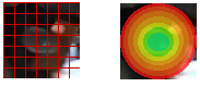
\includegraphics[width=0.9\linewidth]{tradicional/descritores}
    \caption{Regular block grid (left) and concentric rings descriptors (right).}
    \label{fig:descriptors}
    \end{figure}

    \subsection{Regular block grid feature extractor}
      This descriptor divides the candidate window into 7x7 blocks, as illustrated in Figure \ref{fig:descriptors}. The mean value of pixels belonging to each block is calculated, generating a 7x7 matrix of mean pixel intensities. Next, the mean value of the central block is subtracted from the matrix. Finally, the resulting matrix histogram is calculated with 32 bins. The histogram vector, with 32 dimensions, is considered the feature vector, which sums up to 49 (number of blocks).

    \subsection{Concentric rings feature extractor}
       First the candidate window is divided in 18 annulus, or rings, with equal distance between the inner and outer radius and whose center coincides with the window center. Then for each ring the mean of the pixels that belong to it is calculated, resulting in a 18 dimensional vector of mean pixel intensity. Next, the mean value of the inner ring (lower radius equals zero) is subtracted from this vector. Following, we perform a discrete differentiation of this vector (subtraction between adjacent dimensions) to enunciate the differences in rings mean values, resulting in a 15-dimensional feature vector.

    \subsection{SVM classifier}
      We use a binary SVM classifier with Radial Basis Function (RBF) kernel \cite{rbfkernel} to validate the candidates. Recall that the kernel parameter $\sigma$ along with the SVM hyper-parameter $C$ control the trade-off between training performance and generalization on unseen data. Higher $C$ values penalize training set errors, while lower values offer a more general performance on the test set, conversely, the $\sigma$ parameter penalizes in the inverse manner.

      To choose the appropriate values of the hyper-parameters $C$ and $\sigma$ we use a 5 fold cross-validation process, scoring the \textit{precision} metric \cite{evaluationMetrics}. Then a complete training using the entire training dataset, composed by 9894 negative samples and 1222 positive samples is performed. The dataset was generated from video samples collected at the factory during a experiment to test camera positions (placed at a height of 6m), each sample of the dataset is a window cut from a depth frame. These cuts are obtained with the candidate selection procedure presented in Section \ref{sec:candidates} and are manually labeled as positive (human) or negative (not human).

      The SVM classifier was implemented in Python using the Scikit-learn \cite{scikit-learn} toolkit.


\section{Deep learning based solution}
\label{sec:deep}

    Neural networks can be used to perform robust classification with complexity varying according to the network structure and depth. We use and evaluate two deep structures: multilayer perceptron (MLP) and convolutional neural networks (CNN). In our solution for both approaches, the candidate is resized to a 60x60 window and directly fed to the classifier, without any feature-extraction process. We can consider that the model itself will encode a feature set in the first layers of the network, with the final layer doing the classification process and outputing a single probability of that candidate being a human. The diagram would be the same as presented in Figure \ref{fig:system-diagram} without the feature extraction block and with a real valued output probability.

    \subsection{Multilayer perceptron}toolkit
        The MLP structure is composed by units organized in layers. Every unit in a single layer is connected to every unit on the following layer. Each unit calculates its output by summing of its inputs, weigthed by the connections parameters, and then applying an activation function $\phi(x)$. Each output is forward propagated through the network from the input layers, through the hidden layers until the output layer.

        We use a structure with 3600 input units (60x60 pixels), 512 and 256 units in the hidden layers and a single unit in the output layer, as seen in Figure \ref{fig:diag-mlp}. The hidden layers, shown in yellow, use the RELU \cite{nair2010relu} activation function to avoid the vanishing gradient problem. The single output unit uses a sigmoid activation function to reproduce a probabilistic output.

        \begin{figure}
        \centering
        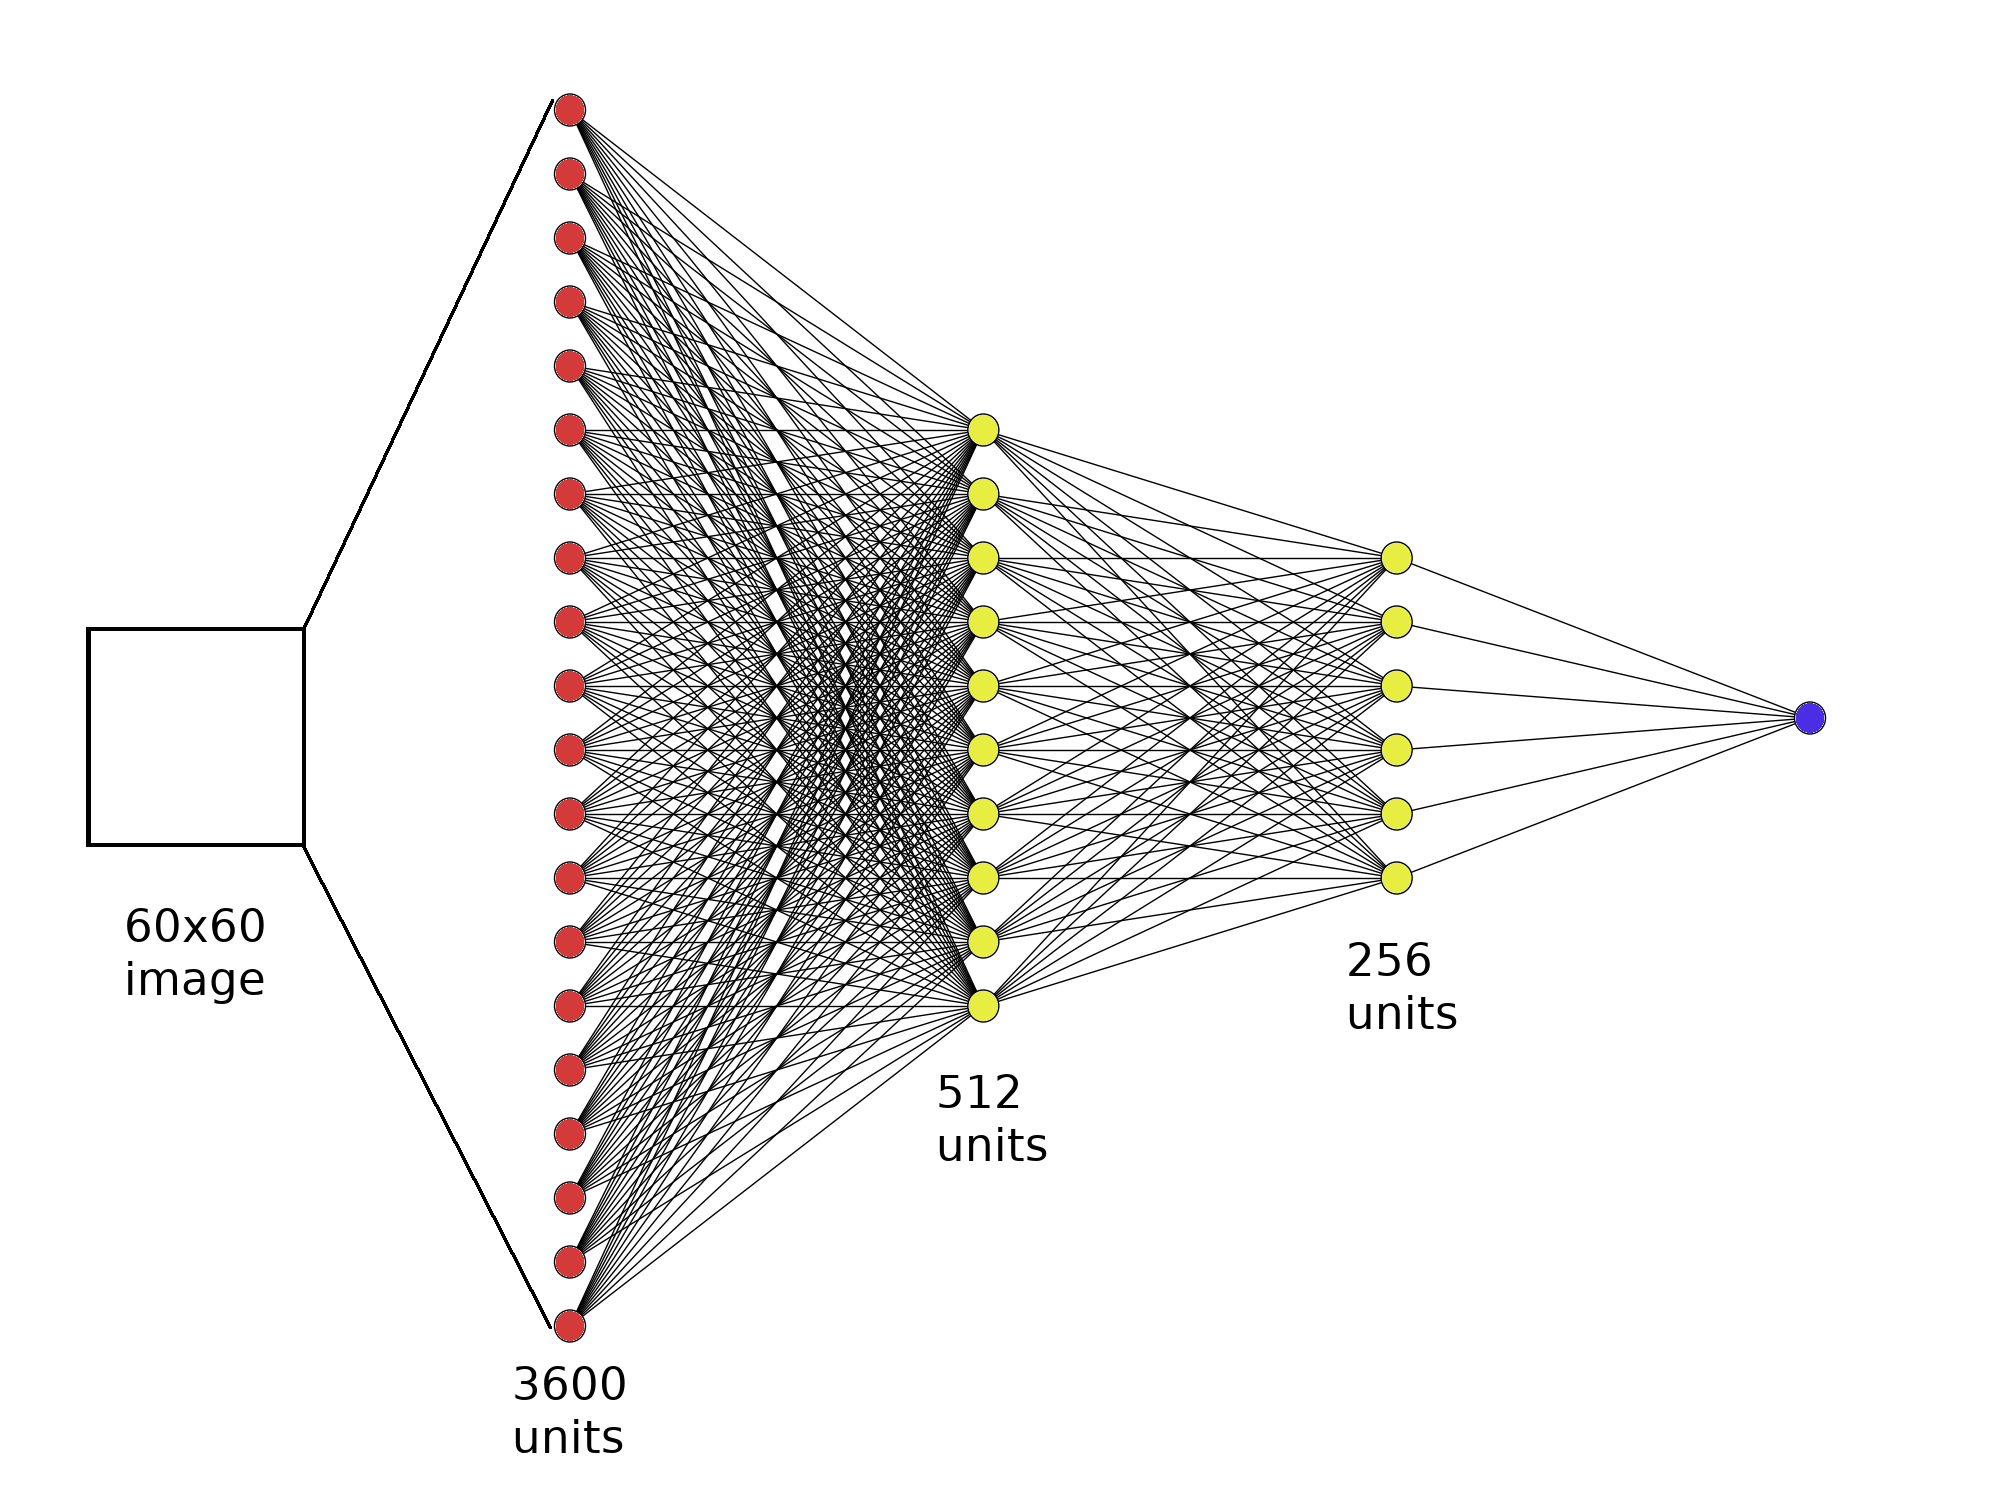
\includegraphics[width=0.8\linewidth]{diagram/diag-mlp.png}
        \caption{MLP network structure.}
        \label{fig:diag-mlp}
        \end{figure}

    \subsection{Convolutional neural network}
         In images there are strong local correlation of pixels, so it is not necessary that every unit in each layer is connected to every unit in the following layer, but just to a few local neighbours. This local connectivity is achieved through the convolution of a given layer with a bank of filters. In this sense, convolutional neural networks are a derivation of MLP and, in general, give a better model for images by reducing the number of parameters thus helping to generalize.

        Our CNN structure, depicted in Figure \ref{fig:diag-cnn}, is composed by a 3x3 convolution layer with 16 feature maps (filters), followed by a 3x3 max pooling layer, then flattening resulting in 5776 (16x19x19) units followed by a 128-units dense layer to perform classification, and finally by a single output unit that gives a probabilistic output. Again, the hidden layers use RELU activation and the output unit uses sigmoid activation.

        \begin{figure}
        \centering
        \includegraphics[width=0.9\linewidth]{diagram/diag-cnn.png}
        \caption{CNN network structure.}
        \label{fig:diag-cnn}
        \end{figure}

    \subsection{Implementation}
        The training process consists of minimizing an objective function, in this case, the binary cross-entropy function \cite{DLbook}, also known as logloss. Its use is justified by the probabilistic nature of the output layer. The optimization method used is a variation of Batch Stochastic Gradient Descent (B-SGD) called Adam \cite{kingma2014adam}, which uses an adaptive learning rate based on momentum considerations (gradient based) for each parameter.

        Since deep models require a larger training set, we extended the SVM training set to 16898 samples, from which 14966 are negative. A challenge faced during the training phase was the impossibility of getting a coherent model due to the unbalanced distribution of the dataset: more than 88\% of the samples belonged to the negative class, so the model would classify all the samples as negative and still get a relative high accuracy. To overcome this, we artificially balanced our training set by replicating positive samples until their frequency was the same as the negative class.

        The computer vision task, candidate extraction, resizing, was done in C++ with the OpenCV library. The deep classifier was implemented using Keras \cite{keras} on top of Theano \cite{theano}, allowing GPU acceleration and enabling a fast training process (an epoch per minute).


\section{Results}
\label{sec:results}

    The evaluation uses Receiver Operating Characteristic (ROC) curves \cite{evaluationMetrics} to compare between solutions and parameters. These curves are generated from the probabilistic output of the classifiers used. In the case of SVM which under original formulations is a non-probabilistic classifier, we use a logistic regression formulation \cite{svmProbabilisticOutput} to enable a probabilistic output. The advantage of using such a probabilistic output classifier is the possibility of adjusting the true-positive vs false-positive tradeoff even after training, by choosing the probability threshold above which the sample is considered to be positive.

    To evaluate the solutions proposed on Sections \ref{sec:classical} and \ref{sec:deep}, with their variations, we firstly consider the candidates already extracted from a video sequence, which will be called the test set, thus evaluating only the descriptor and classifier. Figure \ref{fig:result-classifiers} shows the performance of the classifiers under the test set and a Area Under Curve (AUC) score \cite{evaluationMetrics} (measured up to 10\% of false-positive rate). We can clearly see that deep based classifiers outperform the traditional hand-engineered feature extraction based approach. Although both MLP and CNN perform similarly, one of them can be chosen depending upon the desired region of operation (higher true-positive rate or lower false-positive rate).

    \begin{figure*}[!t]
    \centering
    \subfloat[]{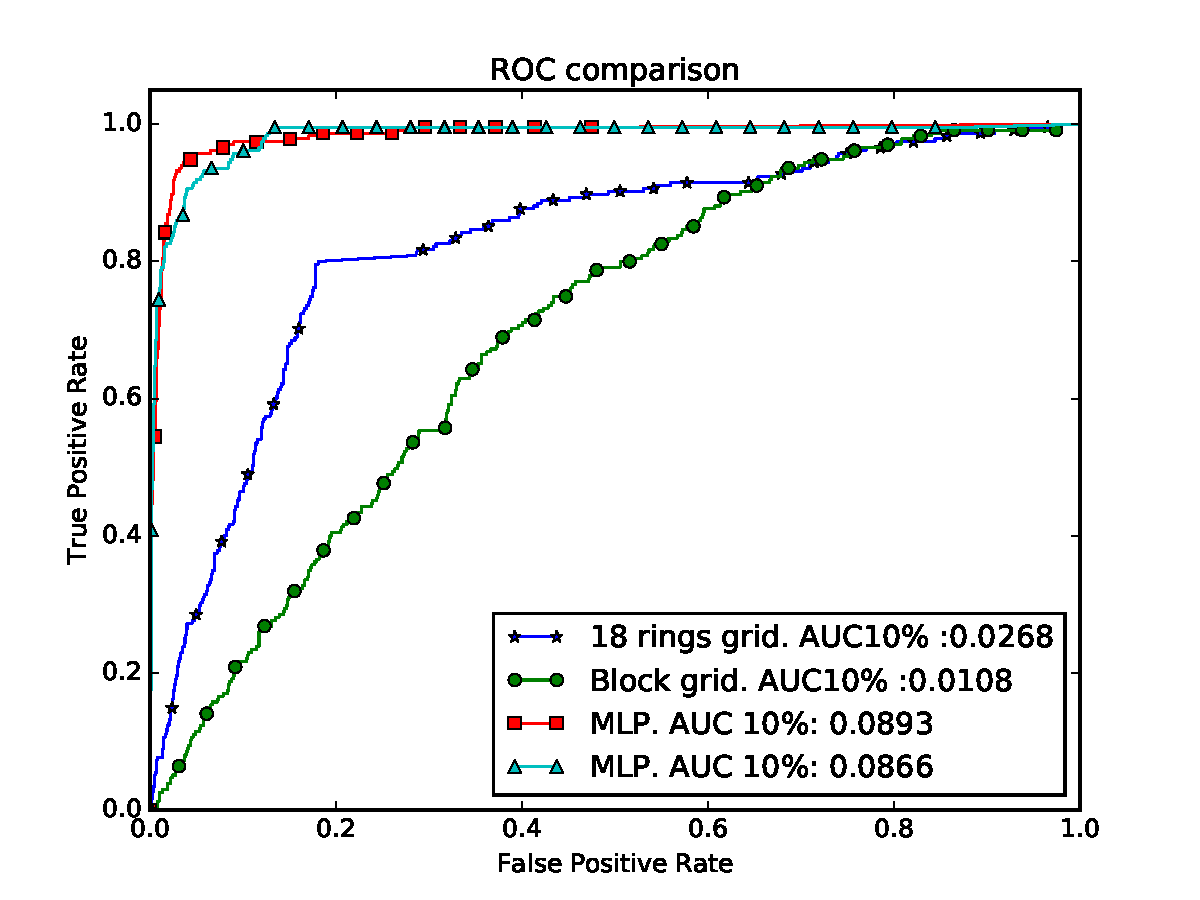
\includegraphics[width=0.45\linewidth]{results/ROC_all.pdf}}%
    \label{fig:result-classifiers-all}
    \hfil
    \subfloat[10 \% interest zone]{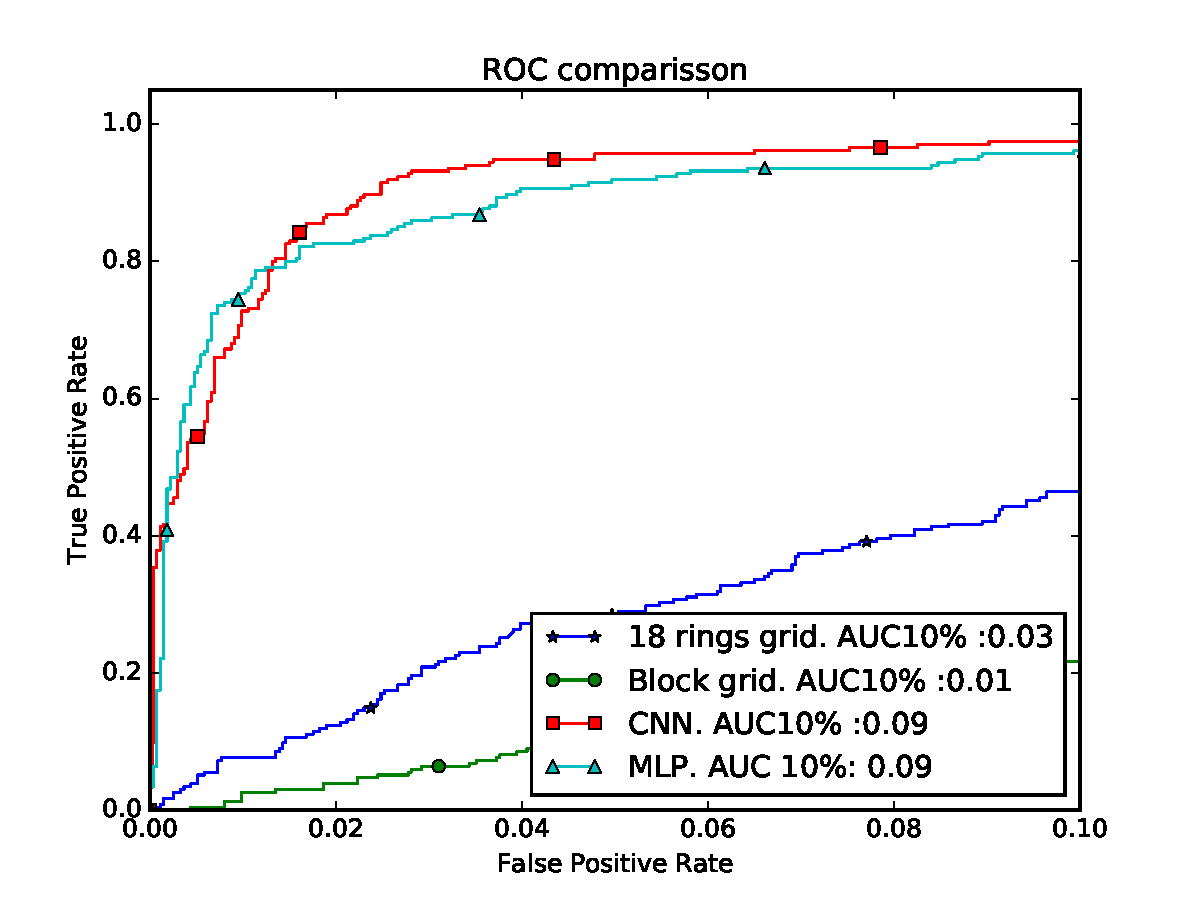
\includegraphics[width=0.45\linewidth]{results/ROC_all_zoom.pdf}}%
    \label{fig:result-classifiers-all-zoom}
    \caption{Classifiers performance.}
    \label{fig:result-classifiers}
    \end{figure*}

    In a second phase we consider the overall system performance, including the candidate extraction step. It is important to note that the performance observed in Figure \ref{fig:result-classifiers} is an upper bound of the overall performance, since now there will be miss-detections from the candidate extraction step. Another consideration is that in this phase the test set is composed of entire frames, so the probability of the frame contain at least one head could be calculated using
    \begin{equation}
    P[y=1] = 1 - \prod_i^n (1-p_i)
    \end{equation}
    where $y$ is a random variable valued 1 if there are humans in the scene or 0 otherwise, $n$ is the number of candidates and $p_i$ is the classifier output of candidate $i$. Figure \ref{fig:result-system} shows the overall system performance using this formulation with the combinations of MLP and CNN classifiers with coarse and fine scales of candidate extraction windows.

    The results show that on a coarse scale detector, the MLP and CNN classifiers have similar performance, because the candidates that get extracted have similar outputs. However, on a fine scale detector, many more candidates are detected so there are more samples to explore the performances of the two classifiers, showing how the CNN model outperforms MLP.

    \begin{figure*}[!t]
    \centering
    \subfloat[]{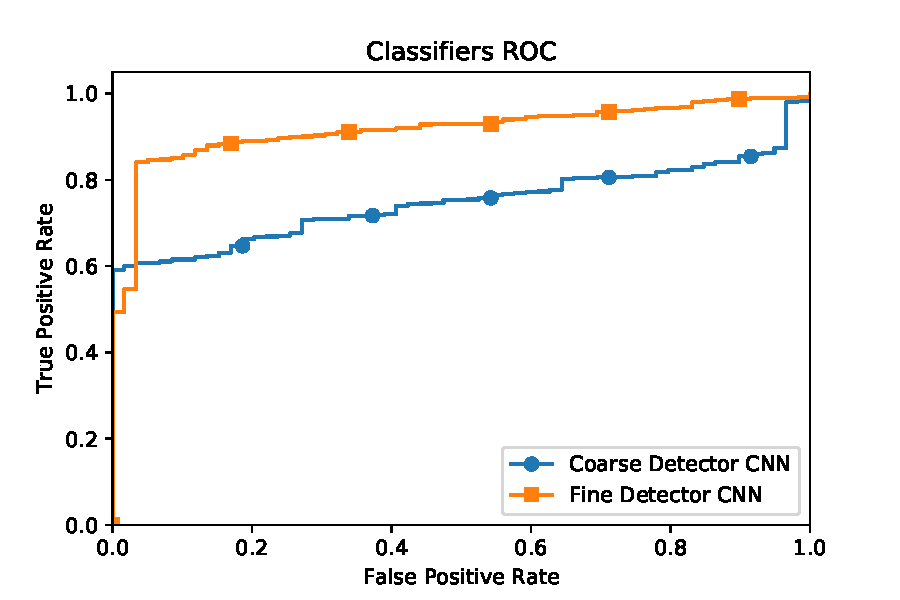
\includegraphics[width=0.45\linewidth]{results/ROC_system.pdf}}%
    \label{fig:result-system-all}
    \hfil
    \subfloat[10 \% interest zone, best results]{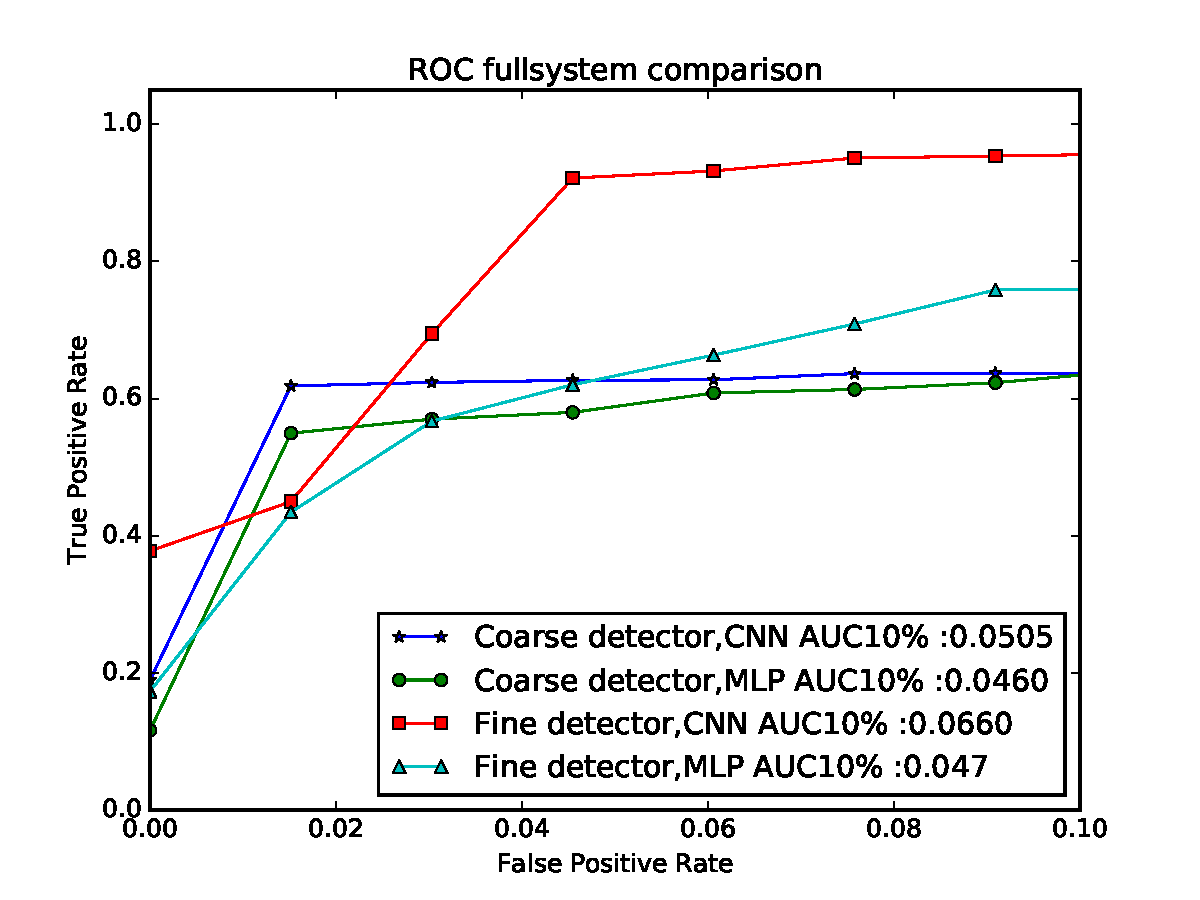
\includegraphics[width=0.45\linewidth]{results/ROC_system_zoom_best.pdf}}%
    \label{fig:result-system-all-zoom}
    \caption{Overall system performance.}
    \label{fig:result-system}
    \end{figure*}

\section{Conclusion}
\label{sec:conclusion}

    This paper investigates two solutions for the human detection problem, one based on traditional computer vision methods and another on deep learning techniques. The results presented in Section \ref{sec:results} show that the last method outperforms traditional hand-engineered feature extraction and classification, although they require a larger training set and have higher complexity, thus requiring more processing power. While deep learning techniques are widely regarded as useful for big datasets, we were still able to achieve good performance, even under a moderate-sized unbalanced dataset.

    One possible direction of future work is investigating a more general CNN structure. Instead of receiving just the candidate window, it would receive the whole depth frame as input and output the probability that frame contains a human. As we saw an improvement of the classification by letting the model choose the best representation of the data, we suspect that allowing the model to access the whole frame as opposed to only small windows possibly containing humans will improve the overall system performance.
